%!TEX root = ../dokumentation.tex

\chapter{Untersuchung der Bewegungen des Roboters}
Um dem Roboter sinnvolle Steuerungsbefehle geben zu können, ist es nicht nur wichtig die Bewegung des Pucks richtig vorhersagen zu können. Vielmehr muss man, vor allem um bei einem Angriffsschlag den Puck zu treffen, auch wissen wie der Schläger sich bewegt. Aus diesem Grund haben wir eine ausführliche Untersuchung der Roboterbewegung durchgeführt, welche in diesem Kapitel beschrieben wird. Um die beschriebenen Bewegungen besser nachvollziehen zu können, ist in Abbildung ~\ref{koordintensystem} das zugrundeliegende Koordinatensystem dargestellt. 

\begin{figure}[htbp]
\centering
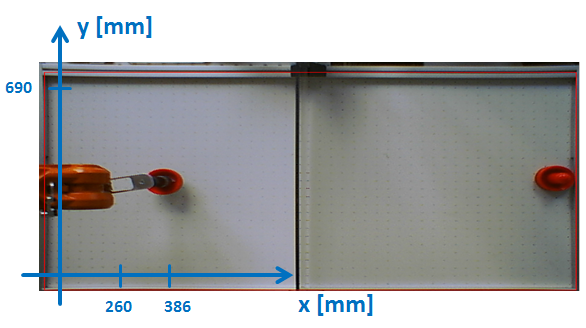
\includegraphics[width=12cm]{Koordinatensystem.png}
\caption{Koordinatensystem des Roboters} 
\label{koordintensystem}
\end{figure}

\section{Versuchsdurchführung}
Um die Bewegung des Roboters zu untersuchen haben wir das Python-Programm \enquote{SpeedTest.py} geschrieben, welches sich in unserem GitHub-Repository zusammen mit den anderen Python-Dateien im Ordner \enquote{airhockey} befindet. 

Dieses besteht im wesentlichen aus der Funktion \enquote{versuch} (siehe Listing ~\ref{speed1}. Diese hat drei Übergabeparameter: Der erste Übergabeparameter muss ein Objekt von der Klasse \enquote{RobotConnection} sein. Die Definition dieser Klasse findet man in der Datei \enquote{Connection.py}. Der zweite Übergabewert ist die Startposition von der aus der Roboter zur Endposition fahren soll, welche man mit dem dritten Übergabeparameter festlegen kann. Diese beiden Werte müssen als zweistelliges Tupel übergeben werden ([x-Koordinate, y-Koordinate]). 

In der ersten While-Schleife wird solange versucht dem Roboter die Koordinaten des Startpunktes zu senden, bis dies erfolgreich war. Anschließend wird in der zweiten While-Schleife gewartet bis der Roboter seine Bewegung beendet hat und somit wieder neue Koordinaten entgegen nehmen kann. Ist dies der Fall, so wird zunächst die aktuelle Zeit in der Variable \enquote{start} gespeichert. Danach werden die Koordinaten des Endpunktes gesendet und wieder gewartet bis der Roboter die Beendigung seiner Bewegung sendet. Dieser Zeitpunkt wird dann in der Variablen \enquote{end} gespeichert. Zum Schluss werden die Messergebnisse noch protokolliert. Dazu werden der Startpunkt, der Endpunkt und die Zeit die zum Abfahren dieser Strecke benötigt wurde (\enquote{end} - \enquote{start}) in die Datei \enquote{speedtest.csv} geschrieben.  
\\
\\
\begin{lstlisting}[caption= Python-Funktion für die Zeitmessung, label=speed1]
def versuch(roboter, startpunkt, endpunkt):
  while not roboter.SendKoordinatesToRoboter(startpunkt):
    pass

  while not roboter.canMove():
    pass
    
  start = time.time()
    
  while not roboter.SendKoordinatesToRoboter(endpunkt):
    pass  
     
  while not roboter.canMove():
    pass
    
  end =time.time()  

  protokoll.write(str(startpunkt[0]) + ";" + str(startpunkt[1]) + ";" + str(endpunkt[0]) + ";" + str(endpunkt[1]) + ";" + str(end - start) + "\n")
\end{lstlisting}

Um in einem Durchlauf mehrere Strecken abfahren zu können, kann die Funktion \enquote{versuch} dann beispielsweise in einer For-Schleife mehrmals aufgerufen werden. In Listing ~\ref{speed2} wird zum Beispiel immer ausgehend vom Ursprung ([0,0]) in einem Abstand von zehn Millimetern alle Punkte der Grundlinie (x=0) abgefahren.    
\\
\begin{lstlisting}[caption=Abfahren der Grundlinie, label=speed2]
for y in range(0, 691, 10):
  versuch(roboter, [0, 0], [0, y])
\end{lstlisting} 

\section{Versuchsauswertung}
Dadurch dass die Messwerte als \enquote{Comma-separated values} gespeichert werden, ist es einfach möglich diese Csv-Datei in einem Tabellenkalkulationsprogramm wie beispielsweise Ecxel zu öffnen. 

Zur Auswertung wurde zunächst der Messtabelle eine weitere Spalte mit der jeweils zurückgelegten Strecke hinzugefügt. Diese wurde mit folgender Formel berechnet: 

\begin{equation}
\Delta s=\sqrt{(x_{end}-x_{Start})^{2}+(y_{end}-y_{Start})^{2}}
\end{equation} 

Die zurückgelegt Strecke wurde dann über der dafür jeweils benötigten Zeit in einem Diagramm eingetragen. Auf diese Weise wird  einerseits der Zusammenhang der beiden Größen anschaulich dargestellt. Zum anderen ist es auch möglich eine Trendlinie durch die Punkte zu legen und sich deren Gleichung angeben zu lassen. Auf diese Weise gelangt man zu einer mathematischen Beschreibung, die den Zusammenhang zwischen Weg und Zeit approximiert. Wie gut eine solche Näherung ist, kann durch das Bestimmtheitsmaß ($ R^2 $)angegeben werden. Dabei handelt es sich um ein Maß aus der Statistik für den erklärten Anteil der Varianz einer abhängigen Variablen durch ein statistisches Modell. \cite{wiki:2016}

Auf diese Weise wurden nun unterschiedliche Bewegungen des Roboters ausgewertet. Dabei zeigte sich, dass sich die Bewegungen des Roboters in den meisten Fällen sehr gut mit einer linearen Trendlinie beschreiben lassen. So konnten die Bewegungen entlang der y-Achse (siehe ~\ref{yAchse}) und entlang der x-Achse (siehe ~\ref{xAchse}) durch eine lineare Trendlinie angenähert werden, deren Bestimmtheitsmaß über 99\% liegt. 

\begin{figure}[htbp]
\centering
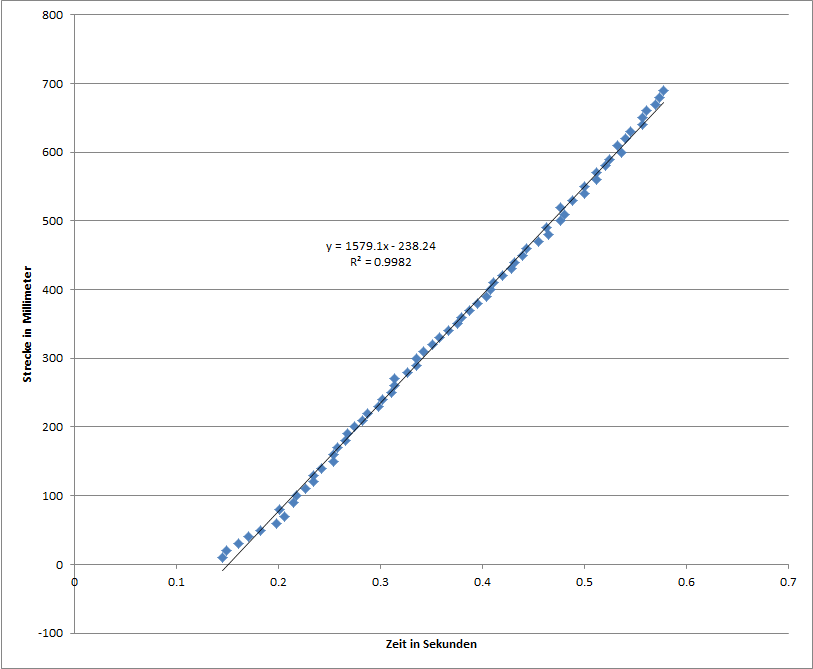
\includegraphics[width=12cm]{grundlinie.png}
\caption{Bewegung entlang der y-Achse auf der Grundlinie} 
\label{yAchse}
\end{figure}      

\begin{figure}[htbp]
\centering
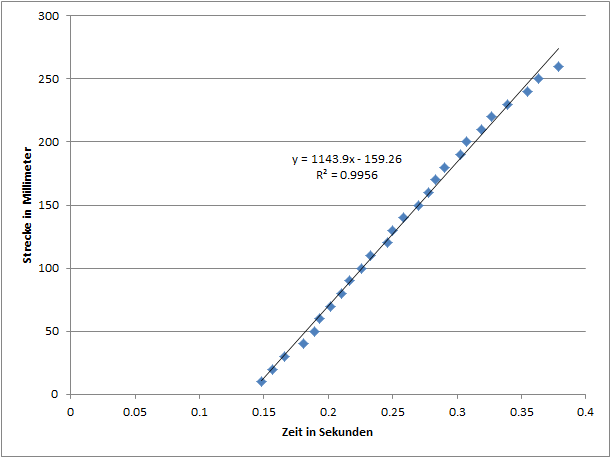
\includegraphics[width=12cm]{xRichtung.png}
\caption{Bewegung entlang der x-Achse bei y = 570} 
\label{xAchse}
\end{figure} 

Bei Diagonal-Bewegungen fiel auf, dass es sich dabei zwar auch um einen linearen Zusammenhang zwischen Weg und Zeit handelt (siehe ~\ref{diagonal}), dieser sich jedoch nicht ganz so genau mathematisch darstellen lässt ($ R^2 < 0,99 $). Des weiteren fiel auf, dass sich die die Steigungen und y-Achsenabschnitte der Geraden-Gleichung sehr stark unterscheiden ja nachdem wo man den Startpunkt wählt und wie man die x- bzw. y- Koordinaten der Endpunkte bei einem Durchlauf variiert. 


\begin{figure}[htbp]
\centering
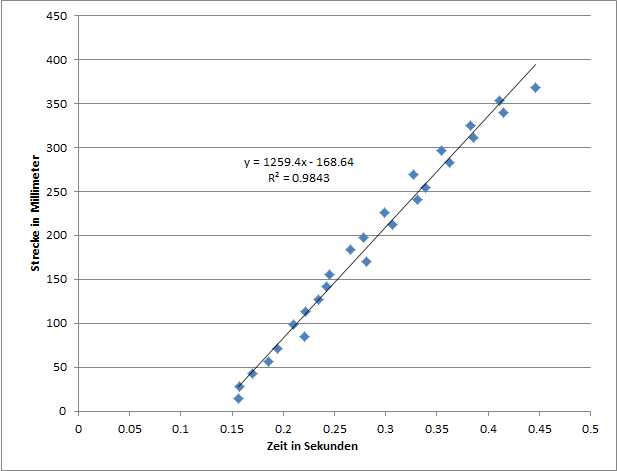
\includegraphics[width=12cm]{diagonal.png}
\caption{Diagonalbewegung} 
\label{diagonal}
\end{figure} 

Wir haben uns deshalb dazu entschlossen, dass wir den Schläger nur auf festgelegten Bahnen fahren lassen. So wird eine Diagonal-Bewegung aufgeteilt in zwei Bewegungen: Zunächst eine Bewegung entlang der y-Achse auf der Grundlinie und anschließend eine Bewegung entlang der x-Achse. 

Zur Berechnung der Zeit, die der Roboter benötigt, um eine gewisse Strecke $ \Delta y $auf der Grundlinie zurückzulegen, kann die Gleichung der linearen Trendlinie verwendet werden (siehe Abb. ~\ref{yAchse}). Diese muss nur etwas umgestellt werden und man erhält folgende Gleichung zur Berechnung von $ t_y $ bei gegebenem $ \Delta y $:

\begin{equation}
t_y =\frac{\Delta y + 238,4}{1579,1}
\end{equation} 

Die Berechnung der Zeit, die der Roboter benötigt um eine Strecke entlang der x-Achse zurückzulegen, gestaltet sich etwas schwieriger. Es hat sich nämlich gezeigt, dass Steigung und y-Achsenabschnitt der unterschiedlichen Geradengleichungen abhängig von der y-Koordinate ist, an der die Bewegung ausgeführt wird. Aus diesem Grund wurde eine Messung durchgeführt, bei der für 25 verschiedene y-Koordinaten die Bewegung entlang der x-Achse untersucht wurde. Dabei wurde für jede y-Koordinate jeweils die Gleichung der linearen Trendlinie bestimmt. Daraufhin wurden die Steigungen und y-Achsenabschnitte dieser Geradengleichungen über ihren entsprechenden y-Koordinaten in Diagramme eingezeichnet (siehe Abb. ~\ref{anstieg} und Abb. ~\ref{offset}). Dabei zeigte sich, dass die Abhängigkeiten dieser beiden Größen zur y-Koordinate jeweils durch ein Polynom zweiten Grades annähern kann. Mit den entsprechenden Trendlinie-Gleichungen kann dann die Steigung und der y-Achsenabschnitts bei vorgegebener y-Koordinate bestimmt werden. 

\begin{figure}[htbp]
\centering
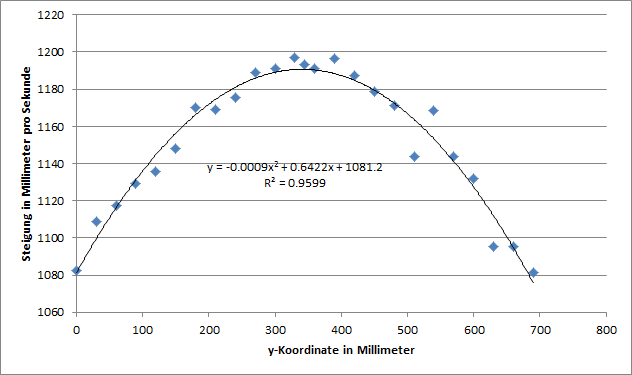
\includegraphics[width=12cm]{anstieg.png}
\caption{Zusammenhang zwischen y-Koordinate und Steigung der Trendlinie} 
\label{anstieg}
\end{figure}

\begin{figure}[htbp]
\centering
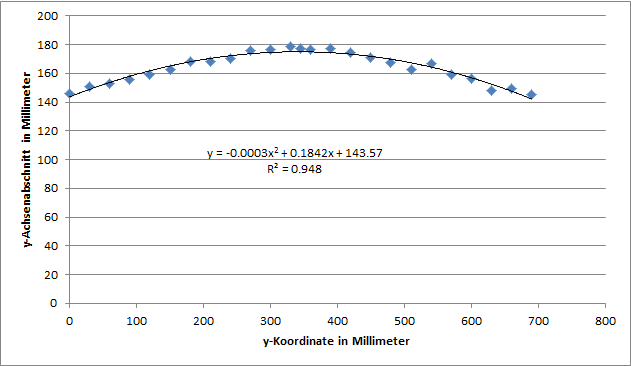
\includegraphics[width=12cm]{offset.png}
\caption{Zusammenhang zwischen y-Koordinate und y-Achsenabschnitt der Trendlinie} 
\label{offset}
\end{figure}

\begin{figure}[htbp]
\centering
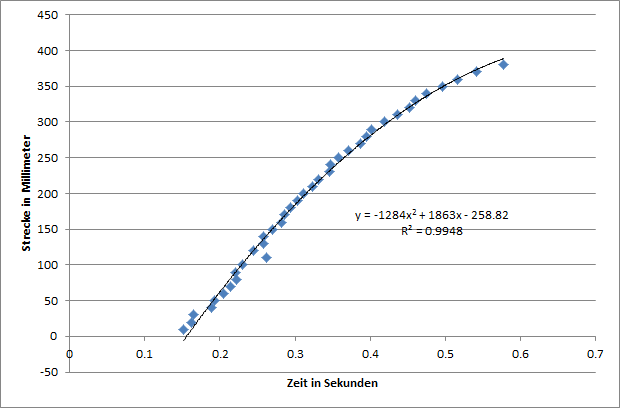
\includegraphics[width=12cm]{mitte.png}
\caption{Bewegung entlang der x-Achse bei y = 345} 
\label{mitte}
\end{figure}
  
Beim Airhockey spielen fiel auf, dass der Puck häufig in eine Pendelbewegung zwischen den beiden langen Banden verfällt. Da die Reichweite des Roboter in y-Richtung jedoch nur 260 mm beträgt, konnte er den Puck oft nicht erreichen und man musste um weiterspielen zu können entweder lange warten, bis der Puck von alleine wieder in unsere Hälfte glitt, oder man musste den Puck mit einem Zollstock anstupsen. 
Da die Reichweite des Roboter in der Mitte des Spielfeldes (bei y = 345) um einiges höher ist als an den Rändern, nämlich 386 mm, wurde eine Strategie ergänzt um einen besseren Spielfluss zu erreichen. Diese sieht vor, dass sobald eine Pendelbewegung vorliegt der Schläger in die Mitte gefahren wird. Von da aus kann er sich dann weiter nach vorne bewegen als sonst. 
Bei der Untersuchung der Bewegung in x-Richtung an dieser Stelle (y=345) fiel auf, dass sich die Bewegung für diese längere Strecke nun nicht mehr gut genug durch eine lineare Trendlinie approximieren lässt (siehe Abb. ~\ref{mitte}). Vielmehr musste man hier ein Polynom zweiten Grades verwenden. Um an dieser Stellen nun für eine gegebene Strecke $ \Delta y $ die entsprechende Zeit $ t_y $ berechnen zu können, musste die Gleichung der Trendlinie noch entsprechend umgeformt werden. Dabei ergab sich folgende Gleichung:

\begin{equation}
t_y = \dfrac{-1863+\sqrt{1893^2-4*(-1284)*(-258,82-\Delta y)}}{2*(-1284)}
\end{equation} 

\section{Schlussfolgerungen}
Ohne diese Untersuchung der Roboterbewegung wäre es nicht möglich gewesen einen Angriffsschlag zu implementieren. Die Approximation die hierbei erarbeitet wurden, sind in sofern ausreichend, dass der Roboter meistens den Puck trifft sobald er einen Angriffsschlag durchführt. 

Die Beschränkung der Roboterbewegungen auf Bewegungen entlang der x- und y-Achse ist jedoch sehr stark und lässt kaum ausgefeiltere Strategien zu. Außerdem fiel auf, dass der Roboter den Puck bei einer Pendelbewegung häufig verfehlt, obwohl extra für diesen Fall eine eigene Funktion zur Berechnung der benötigten Zeit erarbeitet wurde. 

Zur Behebung dieser beiden Probleme könnten man anstatt kontinuierliche Werte für die Koordinaten zu verwenden nur diskrete Werte zulassen. Zum Beispiel für die x-Koordinate nur die Werte 0,30,60, ... ,690 und für die y-Koordinate nur 0,26,52, ... ,260. Man könnte dann mit dem Schläger 254 verschieden Positionen anfahren. Misst man anschließend von jeder Position aus wie lange man benötigt um von hier aus zu allen anderen Positionen zu gelangen, könnten man die entsprechenden Zeiten in eine Lookup-Table eintragen. Mit einer solchen Implementierung wären dann auch Diagonal-Bewegungen ohne weiteres möglich. Die Erzeugung einer solchen Lookup-Table ist jedoch extrem aufwendig. Es wäre deshalb ratsam zunächst zu testen, ob man dadurch merkliche Verbesserungen erzielen kann. Anbieten würde sich dafür die Bewegung in x-Richtung in der Mitte des Tisches, da dafür sowieso schon einen eigene Funktion verwendet wird und man dabei eine Verbesserung auch deutlich merken sollte. 